\documentclass[11pt]{article}
\usepackage{fullpage}
\usepackage{amsmath, multirow}
\usepackage{amssymb}
\usepackage{amsthm}
\usepackage{xcolor}

\usepackage{graphicx}
\usepackage{listings}
\lstset{language=Python, numbers=left, basicstyle=\ttfamily, keywordstyle=\color{blue}, showstringspaces=false}

\newcommand{\dist}{\mathrm{\bf dist}}
\pagestyle{empty}

%\parskip .125in

\begin{document}
\begin{center}
{\bf Intro to Computational Math, Fall 2025\\
Homework 6 Sample Solutions}
\end{center}

{\bf Question 1.}

We use the local convergence criterion: if \(g(p)=p\) and \(|g'(p)|<1\), then the fixed-point iteration \(x_{k+1}=g(x_k)\) converges to \(p\) for all \(x_0\) sufficiently close to \(p\). If \(|g'(p)|>1\), then \(p\) is a repelling fixed point and the iteration cannot converge to \(p\) from nearby starts.

\vskip1cm
\noindent\textbf{(a)} \(g(x)=3+x-x^2\), \(p=\sqrt{3}\).
\[
g(p)=3+\sqrt{3}-3=\sqrt{3}=p, \qquad
g'(x)=1-2x, \qquad
g'(p)=1-2\sqrt{3}.
\]
Since \(|g'(p)|=2\sqrt{3}-1>1\), the iteration cannot converge to \(p\).

\vskip1cm
\noindent\textbf{(b)} \(g(x)=\sqrt{1+x}\), \(p=(1+\sqrt{5})/2\).
\begin{align*}
    g(p) &= \sqrt{1+p} \\
    &= \sqrt{1 + \frac{1 + \sqrt{5}}{2}} \\
    &= \sqrt{\frac{6 + 2\sqrt{5}}{4}} \\
    &= \sqrt{\frac{1 + 2\sqrt{5} + 5}{4}} \\
    &= \sqrt{\left(\frac{1 + \sqrt{5}}{2}\right)^2} \\
    &= (1 + \sqrt{5})/2 \\
    &= p
\end{align*}
\[
g'(x)= \frac{1}{2\sqrt{1+x}}, \qquad
g'(p)= \frac{1}{2p} = \frac{1}{2(1+\sqrt{5})/2} = \frac{1}{1 + \sqrt{5}} = \frac{1}{\sqrt{5} + 1} \cdot \frac{\sqrt{5} - 1}{\sqrt{5} - 1} = \frac{\sqrt{5}-1}{4}.
\]
Thus \(|g'(p)|=(\sqrt{5}-1)/4 \approx 0.31 <1\), so the iteration converges locally to \(p\).

\vskip1cm
\noindent\textbf{(c)} \(g(x)=-\sqrt{1+x}\), \(p=(1-\sqrt{5})/2\).
\begin{align*}
    g(p) &= -\sqrt{1 + p} \\
    &= -\sqrt{1 + \frac{1 - \sqrt{5}}{2}} \\
    &= -\sqrt{\frac{6 - 2\sqrt{5}}{4}} \\
    &= -\sqrt{\frac{1 - 2\sqrt{5} + 5}{4}} \\
    &= -\sqrt{\left(\frac{1 - \sqrt{5}}{2}\right)^2} \\
    &= (1 - \sqrt{5})/2 \\
    &= p
\end{align*}
\[
g'(x)=-\frac{1}{2\sqrt{1+x}}, \qquad
g'(p)=-\frac{1}{2\sqrt{1+p}}.
\]
Since \(\sqrt{1+p}=-p\), we have \(g'(p)=\frac{1}{2p}\) with \(p<0\), and therefore
\[
|g'(p)|=\frac{1}{2|p|}=\frac{1}{2(\sqrt{5} - 1)/2} = \frac{1}{\sqrt{5} - 1} = \frac{1}{\sqrt{5} - 1} \cdot \frac{\sqrt{5} + 1}{\sqrt{5} + 1} = \frac{\sqrt{5} + 1}{4} \approx 0.80 < 1.
\]
Hence the iteration converges locally to \(p\) and the errors alternate because \(g'(p)<0\).

\vskip1cm
\noindent\textbf{(d)} \(g(x)=x+1-\tan(\pi x)\), \(p=1/4\).
\[
g(p)=\frac{1}{4}+1-\tan\!\left(\frac{\pi}{4}\right)= \frac{1}{4} + 1 - 1 = \frac{1}{4}=p, \qquad
g'(x)=1-\pi\sec^{2}(\pi x), \qquad
g'(p)=1-\pi \left(\frac{1}{\sqrt{2}}\right)^2 = 1 - 2\pi.
\]
Since \(|g'(p)|=2\pi-1>1\), the iteration cannot converge to \(p\).


\newpage



{\bf Question 2.}

\paragraph{Solution.}

The standard forms root finding algorithms are:
\begin{itemize}
    \item (4.3.1) \(f(x)=x^{2}-e^{-x}\). Then \(f'(x)=2x+e^{-x}\). We see only one root in the designated window.
    \item (4.3.2) Define \(f(x)=2x-\tan x\). Then \(f'(x)=2-\sec^{2}x\).
    \item (4.3.3) Define \(f(x)=\sin(\pi x)-2x\). Then \(f'(x)=\pi\cos(\pi x)-2\).
\end{itemize}

\begin{lstlisting}
import numpy as np
import scipy
import matplotlib.pyplot as plt
import warnings


def newton(f, dfdx, x1):
    """
    newton(f, dfdx, x1)

    Use Newton's method to find a root of f starting from x1, where dfdx is the
    derivative of f. Returns a vector of root estimates.
    """
    # Operating parameters.
    eps = np.finfo(float).eps
    funtol = 100 * eps
    xtol = 100 * eps
    maxiter = 40

    x = np.zeros(maxiter)
    x[0] = x1
    y = f(x1)
    dx = np.inf  # for initial pass below
    k = 0

    while (abs(dx) > xtol) and (abs(y) > funtol) and (k < maxiter - 1):
        dydx = dfdx(x[k])
        dx = -y / dydx  # Newton step
        x[k + 1] = x[k] + dx  # new estimate

        k = k + 1
        y = f(x[k])

    if k == maxiter:
        warnings.warn("Maximum number of iterations reached.")

    return x[:k+1]


def check_quadratic_convergence(x, root):
    return [abs((root - x[k+1])/(root - x[k])**2) for k in range(len(x) - 1)]


def f_1(x):
    return x**2 - np.exp(-x)

def f_1_prime(x):
    return 2*x + np.exp(-x)

def f_2(x):
    return 2*x - np.tan(x)

def f_2_prime(x):
    return 2 - 1/(np.cos(x)**2)

def f_3(x):
    return np.sin(np.pi * x) - (2 * x)

def f_3_prime(x):
    return np.pi * np.cos(np.pi * x) - 2


# 4.3.1
x = np.linspace(-2, 2, 400)
plt.plot(x, [f_1(x_) for x_ in x])
plt.axhline(0)
plt.title("4.3.1")
plt.show()

print("4.3.1: ")
r1_native = scipy.optimize.root_scalar(f_1, bracket=[0, 1]).root
print("\tNative Root Solver: " + str(r1_native))
r1_newton = newton(f_1, f_1_prime, 0)
print("\tNewton's Method (4.3.1): " + str(r1_newton[-1]))
print("\tConvergence: " + str(check_quadratic_convergence(r1_newton, r1_native)))


# 4.3.2
x = np.linspace(-0.2, 1.4, 400)
plt.plot(x, [f_2(x_) for x_ in x])
plt.ylim([-1, 1])
plt.axhline(0)
plt.title("4.3.2")
plt.show()

print("4.3.2: ")
r2_native = scipy.optimize.root_scalar(f_2, bracket=[-0.1, 0.1]).root
r2_native_2 = scipy.optimize.root_scalar(f_2, bracket=[1.0, 1.2]).root
print("\tNative Root Solver: " + str(r2_native) + ", " + str(r2_native_2))
r2_newton = newton(f_2, f_2_prime, 0)
r2_newton_2 = newton(f_2, f_2_prime, 1.17)
print("\tNewton's Method (4.3.1): " + str(r2_newton[-1]) + ", " + str(r2_newton_2[-1]))
print("\tConvergence: " + str(check_quadratic_convergence(r2_newton_2, r2_native_2)))


# 4.3.3
x = np.linspace(0.1, 2, 400)
plt.plot(x, [f_3(x_) for x_ in x])
plt.axhline(0)
plt.title("4.3.3")
plt.show()

print("4.3.3: ")
r3_native = scipy.optimize.root_scalar(f_3, bracket=[0.4, 0.6]).root
print("\tNative Root Solver: " + str(r3_native))
r3_newton = newton(f_3, f_3_prime, 0.48)
print("\tNewton's Method (4.3.1): " + str(r3_newton[-1]))
print("\tConvergence: " + str(check_quadratic_convergence(r3_newton, 0.5)))
\end{lstlisting}

Output:
\begin{center}
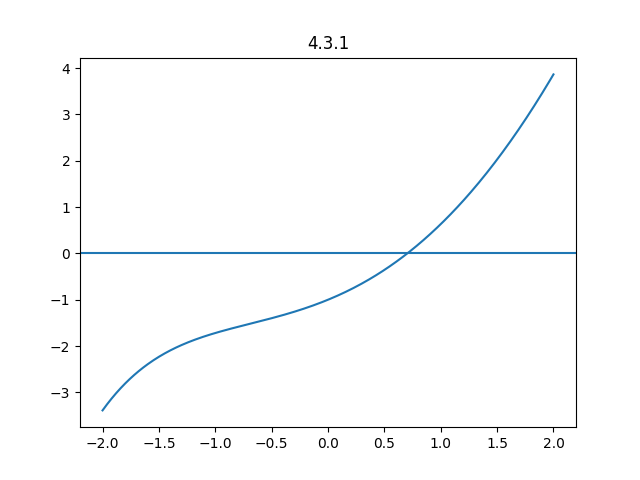
\includegraphics[width=0.3\textwidth]{4.3.1_fig.png} 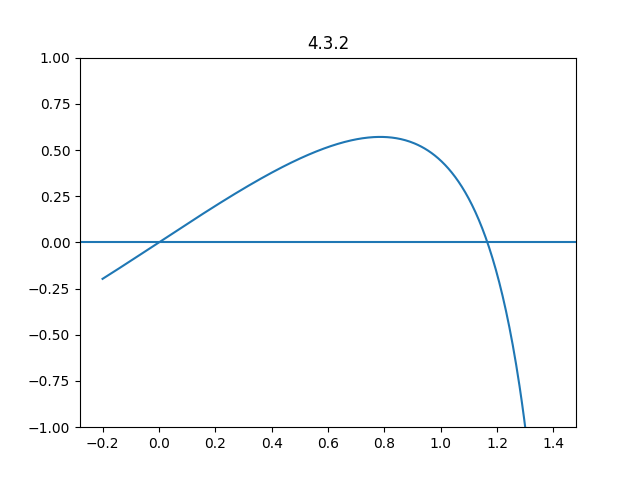
\includegraphics[width=0.3\textwidth]{4.3.2_fig.png} 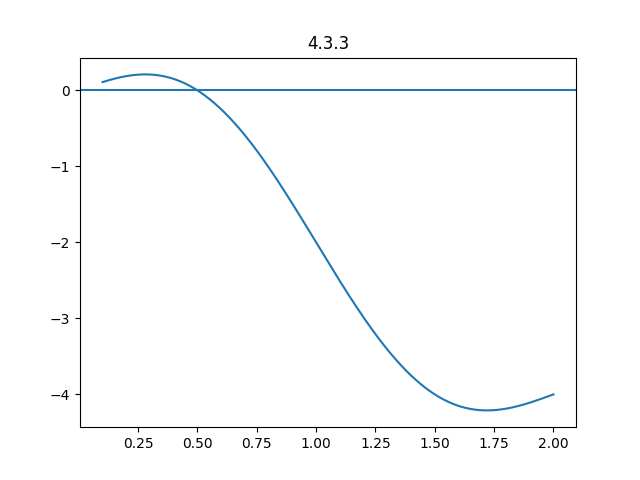
\includegraphics[width=0.3\textwidth]{4.3.3_fig.png}
\end{center}
\begin{verbatim}
4.3.1: 
	Native Root Solver: 0.7034674224983917
	Newton's Method (4.3.1): 0.7034674224983924
	Convergence: [np.float64(0.599217422728741), np.float64(0.33635454147570565),
    np.float64(0.38909813978134344), np.float64(0.3956355764857774),
    np.float64(0.3699508322822683)]
4.3.2: 
	Native Root Solver: 0.0, 1.1655611852072114
	Newton's Method (4.3.1): 0.0, 1.165561185207212
	Convergence: [np.float64(3.3556488241404976), np.float64(3.382160935821295),
    np.float64(3.047408858708234)]
4.3.3: 
	Native Root Solver: 0.49999999999999994
	Newton's Method (4.3.1): 0.5
	Convergence: [np.float64(2.7346921496026972), np.float64(2.4541461985880213),
    np.float64(2.4673634090765035), np.float64(0.0)]
\end{verbatim}

\newpage



{\bf Question 3.}
\[
h(t)=\cos\Big(\tfrac{2\pi}{365}t\Big)+\exp\Big(-\tfrac{1.05}{365}t\Big)+\tfrac{1}{10000}(t-1)^{2}.
\] has derivative
\[
h'(t)=-a\sin(at)-b\exp(-bt)+2c(t-1),\quad a=\tfrac{2\pi}{365},\ b=\tfrac{1.05}{365},\ c=\tfrac{1}{10000},
\]
and second derivative
\[
h''(t) = -a^2\cos(at) +b^2 \exp(-bt) + 2c
\]

\noindent \textbf{(i) Unit-step gradient descent \(t_{k+1}=t_k-h'(t_k)\) from \(t_0=0\).}

Running $10^5$ steps of gradient descent, we see convergence to $97.44873715444463$. The convergence rate for gradient descent is roughly linear. We see this best in the plot of $\log(t^* - t_k)$.

Numerically, this is supported by the theory telling us that the $h(t)$ is Lipschitz within a reasonable bound of the root. For $0 < t < 100$ the derivative term is very close to $0$ and is clearly bounded by $1$ in absolute value.

\begin{center}
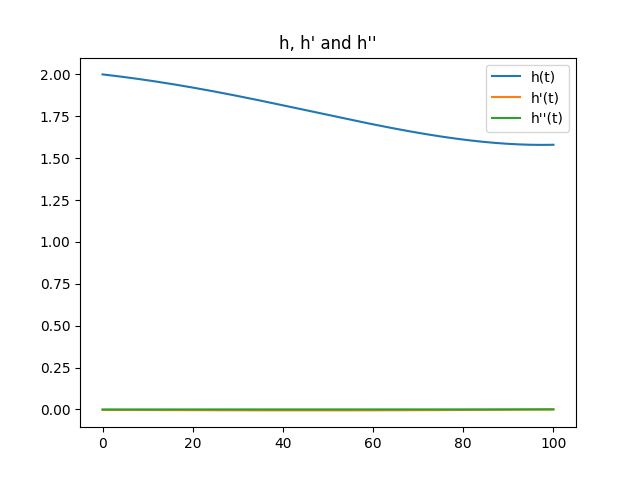
\includegraphics[width=0.45\textwidth]{question3_fcn.png}
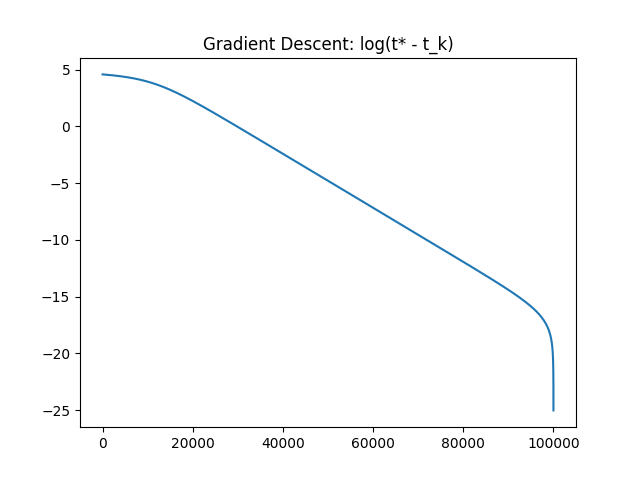
\includegraphics[width=0.45\textwidth]{question3_fig.png}
\end{center}


\noindent\textbf{(ii) Newton’s method on \(h'(t)=0\) from \(t_0=0\).}
Newton on \(f=h'\) is
\[
t_{k+1}=t_k-\frac{f(t_k)}{f'(t_k)}=t_k-\frac{h'(t_k)}{h''(t_k)}.
\]

Because $h''(t) \approx 0$, starting from $t_0 = 0$ which is ``far'' from the root leaves Newton's method to make very large steps initially. The method vastly overshoots the root multiple times before starting to converge. Once near the root, Newton's method rapidly attains the theoretical near quadratic convergence to a value of $97.44873721106528$.

\begin{center}
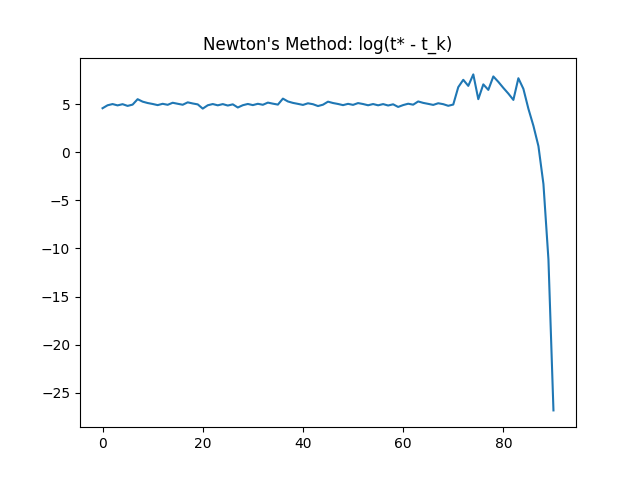
\includegraphics[width=0.45\textwidth]{question3_fig2.png}
\end{center}

\begin{lstlisting}
import numpy as np
import matplotlib.pyplot as plt

def newton(f, f_prime, x0, steps):
    """
    newton(f, f_prime, x0, steps)

    Use Newton's method to find a root of f starting from x0, where f_prime is the
    derivative of f. Returns a vector of root estimates.
    """
    x = np.zeros(steps + 1)
    x[0] = x0
    k = 0
    while (k < steps):
        x[k + 1] = x[k] - f(x[k])/f_prime(x[k])
        k = k + 1
    return x[:k+1]


a = 2.0 * np.pi / 365.0
b = 1.05 / 365.0
c = 1.0 / 10000.0

def h(t):
    return np.cos(a*t) + np.exp(-b*t) + c*((t - 1)**2)

def h_prime(t):
    return -a*np.sin(a*t) - b*np.exp(-b*t) + 2*c*(t - 1)

def h_dprime(t):
    return -a**2 * np.cos(a*t) + b**2 * np.exp(-b * t) + 2*c

t0 = 0
N = 10**5
t_k = [t0]

t = np.linspace(0, 100, 10000)
plt.plot(t, [h(t_) for t_ in t], label='h(t)')
plt.plot(t, [h_prime(t_) for t_ in t], label='h\'(t)')
plt.plot(t, [h_dprime(t_) for t_ in t], label='h\'\'(t)')
plt.title("h, h' and h''")
plt.legend()
plt.show()

for _ in range(N):
    t_k.append(t_k[-1] - h_prime(t_k[-1]))
print(t_k[N])
plt.plot([k for k in range(len(t_k))], np.log(t_k[-1] - t_k))
plt.title("Gradient Descent: log(t* - t_k)")
plt.show()

N = 100
t_k_newton = newton(h_prime, h_dprime, 0, N)
print(t_k_newton[-1])
plt.plot([k for k in range(len(t_k_newton))], np.log(abs(t_k_newton[-1] - t_k_newton)))
plt.title("Newton's Method: log(t* - t_k)")
plt.show()
\end{lstlisting}


\end{document}
